% arara: xelatex
\documentclass[12pt]{article}

% \usepackage{physics}

\usepackage{hyperref}
\hypersetup{
    colorlinks=true,
    linkcolor=blue,
    filecolor=magenta,      
    urlcolor=cyan,
    pdftitle={Overleaf Example},
    pdfpagemode=FullScreen,
    }

\usepackage{tikzducks}

\usepackage{tikz} % картинки в tikz
\usepackage{microtype} % свешивание пунктуации

\usepackage{array} % для столбцов фиксированной ширины

\usepackage{indentfirst} % отступ в первом параграфе

\usepackage{sectsty} % для центрирования названий частей
\allsectionsfont{\centering}

\usepackage{amsmath, amsfonts, amssymb} % куча стандартных математических плюшек

\usepackage{mathtools}
\usepackage{comment}

\usepackage[top=2cm, left=1.2cm, right=1.2cm, bottom=2cm]{geometry} % размер текста на странице

\usepackage{lastpage} % чтобы узнать номер последней страницы

\usepackage{enumitem} % дополнительные плюшки для списков
%  например \begin{enumerate}[resume] позволяет продолжить нумерацию в новом списке
\usepackage{caption}

\usepackage{url} % to use \url{link to web}


\newcommand{\smallduck}{\begin{tikzpicture}[scale=0.3]
    \duck[
        cape=black,
        hat=black,
        mask=black
    ]
    \end{tikzpicture}}

\usepackage{fancyhdr} % весёлые колонтитулы
\pagestyle{fancy}
\lhead{}
\chead{}
\rhead{Econometrics final happiness, 2025-06-24}
\lfoot{}
\cfoot{}
\rfoot{}

\renewcommand{\headrulewidth}{0.4pt}
\renewcommand{\footrulewidth}{0.4pt}

\usepackage{tcolorbox} % рамочки!

\usepackage{todonotes} % для вставки в документ заметок о том, что осталось сделать
% \todo{Здесь надо коэффициенты исправить}
% \missingfigure{Здесь будет Последний день Помпеи}
% \listoftodos - печатает все поставленные \todo'шки


% более красивые таблицы
\usepackage{booktabs}
% заповеди из докупентации:
% 1. Не используйте вертикальные линни
% 2. Не используйте двойные линии
% 3. Единицы измерения - в шапку таблицы
% 4. Не сокращайте .1 вместо 0.1
% 5. Повторяющееся значение повторяйте, а не говорите "то же"


\setcounter{MaxMatrixCols}{20}
% by crazy default pmatrix supports only 10 cols :)


\usepackage{fontspec}
\usepackage{libertine}
\usepackage{polyglossia}

\setmainlanguage{english}
\setotherlanguages{english}

% download "Linux Libertine" fonts:
% http://www.linuxlibertine.org/index.php?id=91&L=1
% \setmainfont{Linux Libertine O} % or Helvetica, Arial, Cambria
% why do we need \newfontfamily:
% http://tex.stackexchange.com/questions/91507/
% \newfontfamily{\cyrillicfonttt}{Linux Libertine O}

\AddEnumerateCounter{\asbuk}{\russian@alph}{щ} % для списков с русскими буквами
% \setlist[enumerate, 2]{label=\asbuk*),ref=\asbuk*}

%% эконометрические сокращения
\DeclareMathOperator{\rank}{rank}
\DeclareMathOperator{\Cov}{\mathbb{C}ov}
\DeclareMathOperator{\Corr}{\mathbb{C}orr}
\DeclareMathOperator{\Var}{\mathbb{V}ar}
\DeclareMathOperator{\pCorr}{\mathrm{pCorr}}
\DeclareMathOperator{\col}{col}
\DeclareMathOperator{\row}{row}
\DeclareMathOperator{\hCov}{\widehat{Cov}}
\DeclareMathOperator{\hVar}{\widehat{Var}}

\newcommand{\dExpo}{\mathrm{Expo}} % o is probably great to avoid confusion with exp function
\let\P\relax
\DeclareMathOperator{\P}{\mathbb{P}}

\DeclarePairedDelimiter{\abs}{\lvert}{\rvert}
\DeclarePairedDelimiter{\norm}{\lVert}{\rVert}

\let\H\relax
\DeclareMathOperator{\H}{\mathbb{H}}


\DeclareMathOperator{\E}{\mathbb{E}}
% \DeclareMathOperator{\tr}{trace}
\DeclareMathOperator{\card}{card}

\DeclareMathOperator{\Convex}{Convex}

\newcommand{\SSR}{SS^{\text{res}}}
\newcommand{\SSE}{SS^{\text{expl}}}
\newcommand{\SST}{SST}
\newcommand{\hb}{\hat\beta}
\newcommand{\hy}{\hat y}
\newcommand \cN{\mathcal{N}}
\newcommand \dN{\mathcal{N}}
\newcommand \dBin{\mathrm{Bin}}

\newcommand{\const}{\text{const}}

\newcommand \RR{\mathbb{R}}
\newcommand \NN{\mathbb{N}}





\begin{document}

\begin{enumerate}
    \item Body positive Zmey Gorynych worries about his weight but loves eating young beautiful princesses.
    Each year he makes weight measurements.
    He is very happy when his weight is between $1000$ and $2000$ kilograms.
    Otherwise he is unhappy and does not remember the exact measurement results. 

    Here are his recordings for the last $5$ years $y = (\leq 1000, 1200, 1500, \geq 2000, 1800)$.

    Assume that his weight measurements are uniform on $[0, a]$ and independent.

    \begin{enumerate}
        \item {[7]} Estimate unknown $a$ using maximum likelihood. 
        \item {[3]} Estimate the probability that the next year Zmey Gorynych will be happy about his weight.
    \end{enumerate}
     

\item Consider the following equations for the process \( x_t, y_t \):

\[
\begin{cases}
x_t = 0.5 y_{t-1} + 0.25 x_{t-2} - 0.5 y_{t-2} + u_{1t}, \\
y_t = -0.5 x_{t-1} + 0.5 y_{t-1} + 0.25 x_{t-2} + 0.5 y_{t-2} + u_{2t},
\end{cases}
\]
where \( u_{1t} \) and \( u_{2t} \) are independent white noise processes.

\begin{enumerate}
    \item {[2]} Represent this system of equations in the $VAR(1)$ form for 4-dimensional process. 
    \item {[3]} Are there any stationary solutions?
    \item {[3]} Derive the VECM (Vector Error Correction Model) representation of these equations. 
    \item {[2]} Write out the cointegrating vector.
\end{enumerate}


    \item Consider the multinomial logit model with 3 alternatives $a$, $b$ and $c$. 
    Here we omit index $i$ for observations and just write $y$ instead of $y_i$ for simplicity. 
    The variables $D_a$, $D_b$ and $D_c$ are «disutilities» of the alternatives. 
    The alternative with the lowest disutility is chosen by individiual.
\[
\begin{cases}
v_a, v_b, v_c \sim \dExpo(\lambda=1) \\
D_{a} = v_{a} / 2, \quad D_{b} = v_{b} / 3, \quad D_{c} = v_{c} / 4 \\ 
y = \begin{cases}
a, \text{ if } D_{a} = \min\{D_{a}, D_{b}, D_{c}\} \\
b, \text{ if } D_{b} = \min\{D_{a}, D_{b}, D_{c}\} \\
c, \text{ if } D_{c} = \min\{D_{a}, D_{b}, D_{c}\} \\
\end{cases}
\end{cases}
\]

\begin{enumerate}
    \item {[3]} What is the distribution of $D_a$, $D_b$ and $D_c$?
    \item {[2]} What is the distribution of $\min\{ D_a, D_b, D_c \}$?
    \item {[3]} Derive the probability $\P(y = a)$.
    \item {[2]} Derive the probability $\P(y = a \mid y \neq c)$.
\end{enumerate}



\newpage



\item Consider the following time series model for \( \{y_t\}_{t=1}^T \):
\[
y_t = \alpha + \beta t + u_t, \quad t = 1, \ldots, T
\]
\[
\text{with} \quad u_t = \rho u_{t-1} + \varepsilon_t \quad \text{and} \quad \abs{\rho} \leq 1
\]

where \( \varepsilon_t \) is an i.i.d. error with distribution \( (0, \sigma_\varepsilon^2) \) that is uncorrelated with anything in the past (white noise).

\begin{enumerate}
    \item {[4]} Show that \( y_t \) is trend stationary when \( |\rho| < 1 \) [ie there is a trend stationary solution].

    \item {[3]} Show that \( y_t \) is difference stationary when \( \rho = 1 \).

    \item {[3]} Discuss the importance of distinguishing between trend stationary and difference stationary processes.
\end{enumerate}


\item Consider the equation 
\[
y_t = y_{t-1} + u_t -1.5u_{t-1} + 0.5u_{t-2},
\]
where $(u_t)$ is a white noise process. 

\begin{enumerate}
    \item {[4]} Write this equation in the form $A(L)y_t = B(L)u_t$ with factored polynomial $B(L)$.
    \item {[2]} Provide an example of a stationary solution of the equation if possible.
    \item {[2]} Provide an example of a difference stationary solution of the equation if possible.
    \item {[2]} Provide an example of a non-stationary solution that is not difference stationary if possible.
\end{enumerate}

\newpage

\item Let us consider an analysis on recidivism (probability of re-arrest) among a group of young men in California 
who have at least one arrest prior to 1986. 
The dependent variable, \verb|arr86|, is equal to unity if the man was arrested at least once during 1986, and zero otherwise.
The standard errors are reported in parentheses.

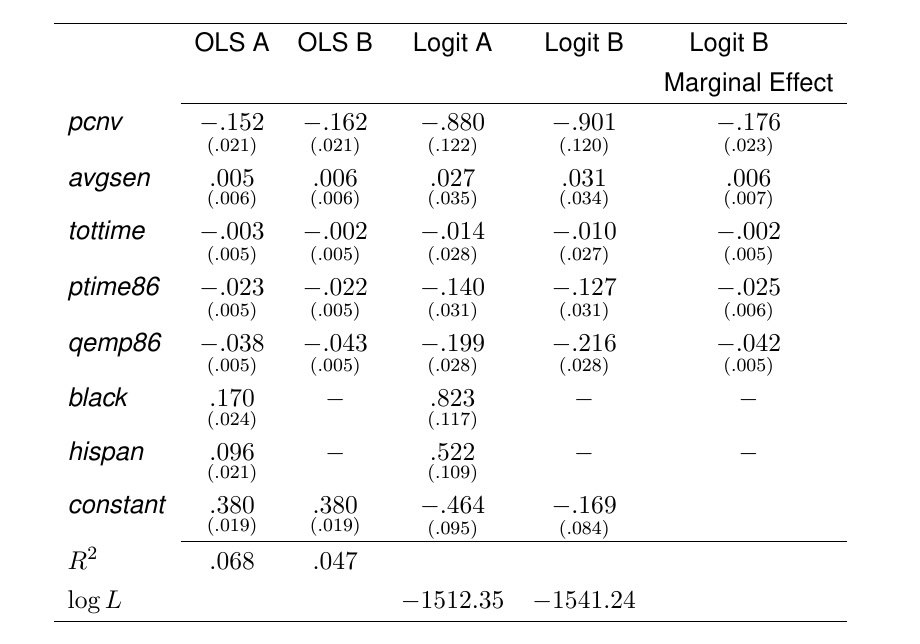
\includegraphics[scale=0.5]{reg_table.jpg}

\verb|pcnv| is the proportion of prior arrests that led to a conviction, \\
\verb|avgsen| is the average sentence served from prior convictions, \\
\verb|tottime| is the months spent in prison since age 18 prior to 1986,  \\
\verb|ptime86| is months spent in prison in 1986, \\
\verb|qemp86| is the number of quarters the man was legally employed in 1986, \\
\verb|black| and \verb|hispan| are two race dummies (white the excluded dummy). 


\begin{enumerate}
    \item {[2]}  Using the OLS B results, 
    what is the estimated effect on the probability of arrest if \verb|pcnv| goes from 0.25 to 0.75 holding everything else constant?
    \item {[2]} It is argued that the linear probability model is not appropriate for explaining the binary variable  \verb|arr86| and a logit regression model has been estimated. 
    Explain how the Logit estimates are obtained.
    \item  {[3]} Using the Logit model results, discuss whether \verb|black| and \verb|hispan| are jointly significant. 
    Clearly indicate the null and alternative hypothesis, the test statistic and the rejection rule.
    \item {[3]} Using the Logit B results, 
    how would you obtain the estimated effect on the probability of arrest if \verb|pcnv| goes from 0.25 to 0.75 for a white man, 
    with characteristics \verb|avgsen=1|, \verb|tottime=1|, \verb|ptime86=0| and \verb|qemp86=2|. 
    A clear explanation of what calculations are required is sufficient.
\end{enumerate}




\end{enumerate}

\end{document}
